\documentclass[11pt,aps,preprint,nofootinbib,superscriptaddress,tightenlines]{revtex4-2}
\usepackage{amsmath,amssymb,bm,mathtools,graphicx}
\usepackage{xcolor}
\definecolor{darkblue}{RGB}{0,0,160}
\usepackage[colorlinks=true,linkcolor=darkblue,citecolor=darkblue,urlcolor=darkblue]{hyperref}

\def\st{\begin{equation}}
\def\stp{\end{equation}}
\def\Eq#1{eq.~(\ref{#1})}
\def\Sect#1{Sect.~\ref{#1}}
\def\Fig#1{Fig.~\ref{#1}}
\newcommand{\avg}[1]{\langle #1\rangle}
\let\oldparagraph\paragraph
\renewcommand{\paragraph}{\par\bigskip\oldparagraph}

\begin{document}

\title{The first NERSC campaigns: stability, heating and equilibrium correlators}
\author{D.~Teaney}
\affiliation{Department of Physics and Astronomy, Stony Brook University,
Stony Brook, New York 11794, USA}
\date{\today}

\begin{abstract}
Three campaigns of the full stochastic scheme (Hamiltonian step plus the stochastic
viscous step in the particle representation) were run on Perlmutter on 8--9 November
2026: a stability scan in the thermal velocity and $\lambda$ (\texttt{first},
\texttt{first\_det}), and equilibrium ensembles in boxes $L=1.2$ and $2.4$, once with the
old code and a thermal start (\texttt{first}) and once with the fast code and the
equilibrium start (\texttt{second}).  This note says what was run, what each figure shows
and why it was made, and what we learned.  In short: (i) the runs heat slowly, as $\delta
v^4$ and faster than linearly in time, and $\lambda=1$ blows up between $\delta v=0.078$
and $0.14$; (ii) the transverse momentum correlator is not diffusive but a damped
oscillation, transverse sound of a weakly rigid particle arrangement; (iii) the fast code
and the equilibrium start reproduce the old results.
\end{abstract}

\maketitle

%=============================================================================
\section{What was run}
\label{sec:runs}

\paragraph{The scheme.}  Every run is a uniform two-dimensional conformal fluid
($c_s^2=1/3$, $\eta/s=0.2$) in a periodic box on a hexagonal lattice with $h=0.05$ and
$h/a=2$.  A time step is the leapfrog of the ideal SPH Hamiltonian $H$ between
stochastic viscous steps (stress and residual moves, checkerboard sweeps,
\texttt{stochrep.tex}), with the gradient-corrected change of representation and the
star vote.  The parameter $\lambda$ of the residual move is $\lambda=1$ (detailed
balance: every mode, including the lattice modes, fluctuates) or $\lambda=\infty$ (the
residual is deterministic: the lattice modes are damped without noise and stay cold).
The entropy density $S_0$ sets the size of the fluctuations: the entropy per particle
is $s_a=S_0V_a$ and the thermal velocity per component is
\st
\delta v=\Big(\frac{T}{wV_a}\Big)^{1/2}=s_a^{-1/2},
\stp
\begin{center}
\begin{tabular}{ccc}
\hline
$S_0$ & $s_a$ & $\delta v$ \\ \hline
$10^6$ & $541$ & $0.043$ \\
$3\times10^5$ & $162$ & $0.078$ \\
$10^5$ & $54$ & $0.14$ \\
\hline
\end{tabular}
\end{center}
The time step is $\Delta t=8.66\times10^{-3}$ in all runs.

\paragraph{The campaigns.}  One Slurm array task per realization, $2$ CPUs (one core) each,
in the \texttt{shared} queue; job scripts, commits and commands are stored next to the
output in \texttt{\$SCRATCH/sph/<campaign>/}, and the record is \texttt{nersc/LOG.md}.
\begin{center}
\begin{tabular}{llllll}
\hline
campaign & set & what varies & box & runs & to \\ \hline
\texttt{first} & ref & $S_0=10^6$, $\lambda=1$ and $\lambda=\infty$ & $0.6$ & 16 & $t=200$ \\
 & s3e5 & $S_0=3\times10^5$, $\lambda=1$ & $0.6$ & 16 & $200$ \\
 & s1e5 & $S_0=10^5$, $\lambda=1$ & $0.6$ & 16 & $200$ \\
 & s1e5\_ha3 & $S_0=10^5$, $\lambda=1$, $h/a=3$ & $0.6$ & 16 & $200$ \\
 & s1e5\_hfix & $S_0=10^5$, $\lambda=1$, energy fix & $0.6$ & 16 & failed \\
\texttt{first\_det} & s3e5\_det, s1e5\_det & $\lambda=\infty$, same seeds & $0.6$ & 16+16 & $200$ \\
\texttt{first} & eqL1.2, eqL2.4 & thermal start, old code & $1.2$, $2.4$ & 32+32 & $400$ \\
\texttt{second} & eqL1.2, eqL2.4 & equilibrium start, fast code & $1.2$, $2.4$ & 32+32 & $400$ \\
\hline
\end{tabular}
\end{center}
The boxes $0.6$, $1.2$, $2.4$ hold $N=672$, $2688$, $10560$ particles.  In
\texttt{first} only 12 of the 32 eqL2.4 runs finished within the 8 h limit (the others
were lost, since output was written only at the end); \texttt{second} writes a
checkpoint every 20 minutes and runs about twice as fast per core (\Sect{sec:code}).

\paragraph{The two drivers.}
\begin{itemize}
\item \texttt{stochrep\_hamiltonian.jl} (stability scan) starts from rest with all momenta
zero, and records over time the kinetic energy $\sum_a|\bm m_a|^2$ divided by its
equilibrium value $2(N-1)V_awT$; the smoothed energy $H$ (conserved by the leapfrog);
the sum of the particle energies $\sum_ae_a$ (held fixed in a stochastic step); and the
\emph{local disorder}, the rms change of the distances between original nearest
neighbours in units of $a$.  A disorder above $1$ means the lattice has melted.
\item \texttt{stochrep\_equilibrium.jl} (ensembles) records the Fourier modes of the
momentum density, $\bm M_{\bm k}(t)$, split into the longitudinal and transverse parts
$M_L$, $M_T$, for all $kh\le1.5$, every 2 (L = 1.2) or 4 (L = 2.4) steps.  From them
\st
C_{T,L}(k,\tau)=\frac{\avg{M_{T,L}(\bm k,t+\tau)M^*_{T,L}(\bm k,t)}}{NV_awT},
\stp
averaged over $t>2$, over the vectors $\bm k$ of a shell $|\bm k|=k$, and over the
realizations.  In equilibrium $C(k,0)=1$.  Hydrodynamics predicts
\st
C_T(k,\tau)=e^{-\nu k^2\tau},\qquad
C_L(k,\tau)=\cos(c_sk\tau)\,e^{-\Gamma_sk^2\tau/2},
\qquad \nu=\frac{\eta}{w}=\frac{\eta/s}{T},
\label{hydro}
\stp
with $\Gamma_s=\tfrac43\nu$ (conformal) and here $\nu=2.2\times10^{-3}$.
\end{itemize}

%=============================================================================
\section{Stability scan}
\label{sec:stab}

\paragraph{Purpose.}  The earlier runs (\texttt{fullruns.tex}) at $\delta v=0.14$ melted the
lattice and blew up after $t\approx45$, while at $\delta v=0.043$ they only heated slowly.
The scan locates the limit in $\delta v$, and asks whether the noise in the lattice modes
($\lambda=1$ against $\lambda=\infty$, same seeds) or the resolution ($h/a=3$) is
responsible.

\begin{figure}[t]
\centering
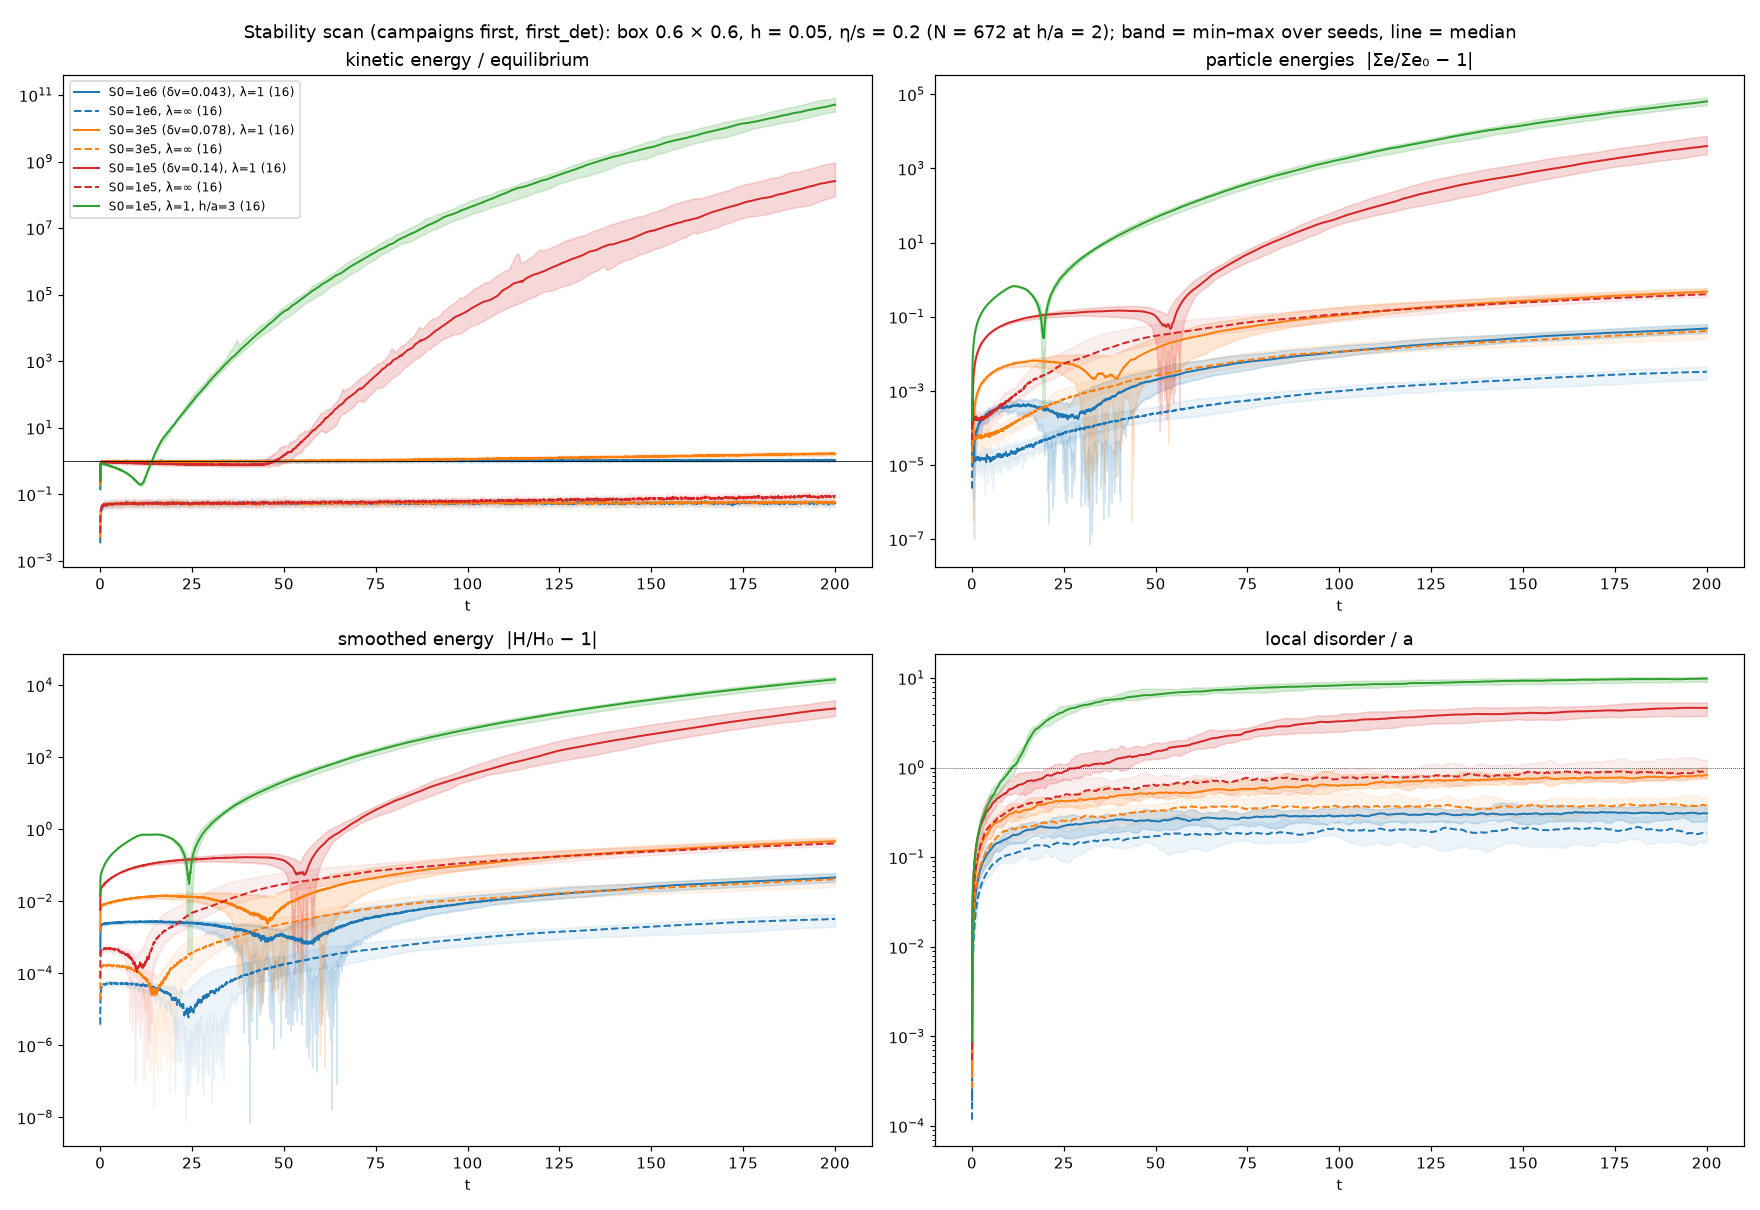
\includegraphics[width=\textwidth]{figs/campaign_first_stability.png}
\caption{Stability scan, box $0.6$, $h/a=2$ unless noted, 16 seeds per set.  Line:
median over the seeds; band: minimum to maximum.  Colour: $\delta v$; solid $\lambda=1$,
dashed $\lambda=\infty$; green: $h/a=3$.  Top left: kinetic energy over its equilibrium
value (the $\lambda=\infty$ runs sit at $\approx0.05$, because only the hydrodynamic
modes are thermalized).  Top right and bottom left: drift of the particle energies and
of the smoothed energy, in magnitude (the dips are sign changes).  Bottom right: local
disorder; the dotted line marks melting.}
\label{fig:stab}
\end{figure}

\begin{figure}[t]
\centering
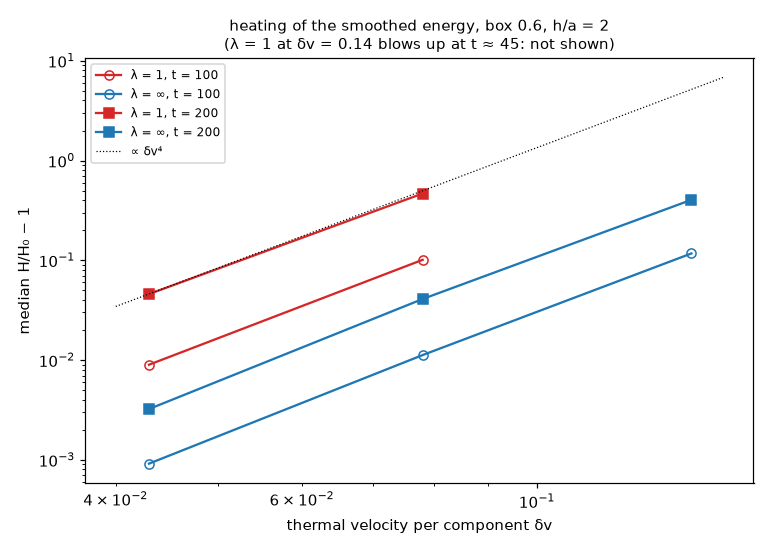
\includegraphics[width=0.65\textwidth]{figs/campaign_first_stability_heating.png}
\caption{The heating of \Fig{fig:stab}: median $H/H_0-1$ at $t=100$ (open) and $t=200$
(filled) against $\delta v$, log--log.  Dotted: $\propto\delta v^4$.}
\label{fig:heat}
\end{figure}

\paragraph{What the figures show.}
\begin{center}
\begin{tabular}{lccccc}
\hline
set ($t=200$, median) & $H/H_0-1$ & KE/eq & disorder & melted & blew up \\ \hline
$\delta v=0.043$, $\lambda=1$ & $0.046$ & $1.06$ & $0.31a$ & 0/16 & 0 \\
$\delta v=0.043$, $\lambda=\infty$ & $0.0032$ & $0.05$ & $0.19a$ & 0/16 & 0 \\
$\delta v=0.078$, $\lambda=1$ & $0.47$ & $1.66$ & $0.83a$ & 1/16 & 0 \\
$\delta v=0.078$, $\lambda=\infty$ & $0.041$ & $0.06$ & $0.38a$ & 0/16 & 0 \\
$\delta v=0.14$, $\lambda=1$ & $2\times10^3$ & $3\times10^8$ & $4.7a$ & 16/16 ($t\approx28$) & 16 \\
$\delta v=0.14$, $\lambda=\infty$ & $0.40$ & $0.09$ & $0.93a$ & 8/16 ($t\approx147$) & 0 \\
$\delta v=0.14$, $\lambda=1$, $h/a=3$ & $1.5\times10^4$ & $5\times10^{10}$ & $9.9a$ & 16/16 ($t\approx11$) & 16 \\
\hline
\end{tabular}
\end{center}
\begin{enumerate}
\item \emph{The limit.}  With $\lambda=1$ the scheme is stable at $\delta v=0.078$ (one
  seed just melting at $t=198$) and blows up at $\delta v=0.14$: the instability sets in
  between $s_a=54$ and $162$.  Once the disorder reaches about $a$ the kinetic energy
  grows exponentially.
\item \emph{The lattice modes.}  $\lambda=\infty$ never blows up, even where its lattice
  disorders to about $a$.  The runaway therefore needs the noise in the lattice modes.
\item \emph{The heating} (\Fig{fig:heat}) grows as $\delta v^4$ for both $\lambda$, and
  $\lambda=1$ heats $10$--$14$ times faster than $\lambda=\infty$ at the same $\delta v$.
  Between $t=100$ and $200$ the drift grows by a factor $4$--$5$: it accelerates,
  roughly as $t^2$, rather than growing linearly.
\item \emph{$h/a=3$} blows up sooner.  At the same $S_0$ it has more, smaller particles,
  so a larger $\delta v$ ($0.21$): not a test at fixed $\delta v$.
\item \emph{The energy fix} (\texttt{SR\_HFIX=1}): the runs failed in the bond weights
  once the lattice had melted, both before and after a fallback was added; the fix does
  not prevent the blow-up.
\end{enumerate}

%=============================================================================
\section{Equilibrium correlators}
\label{sec:corr}

\paragraph{Purpose.}  Test \Eq{hydro}: do the stochastic step and the Hamiltonian step
together reproduce the equilibrium fluctuations ($C(k,0)=1$) and the hydrodynamic decay
of the shear and sound modes?  The boxes are large enough to reach $kh=0.26$ ($L=1.2$)
and $0.13$ ($L=2.4$).  All at $\delta v=0.043$, $\lambda=1$, $t=400$.

\begin{figure}[t]
\centering
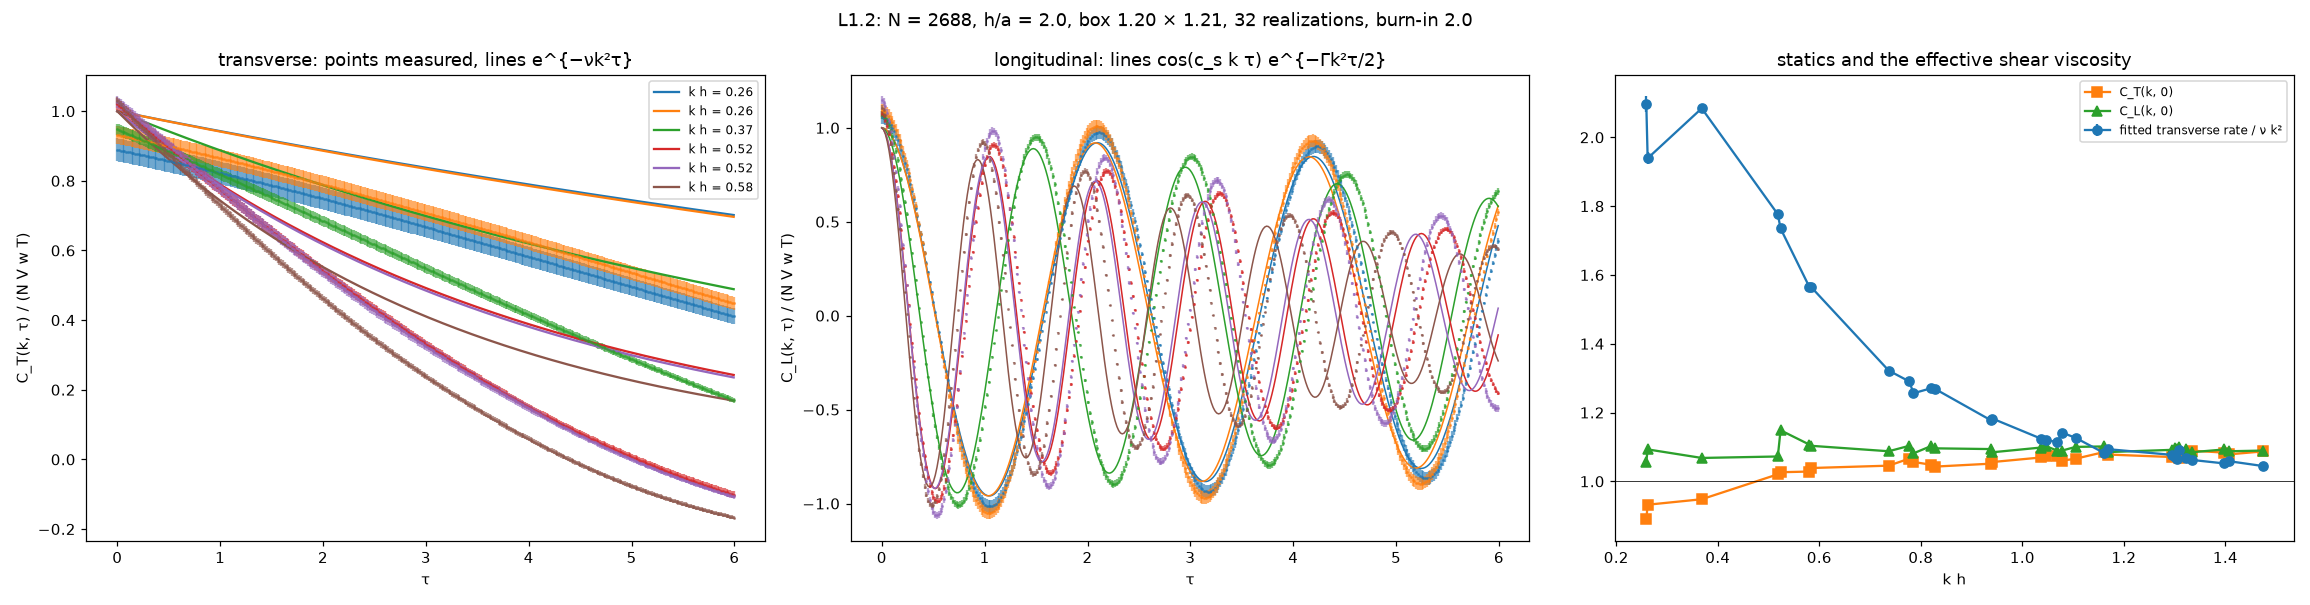
\includegraphics[width=\textwidth]{figs/correlators_L1.2.png}
\caption{Campaign \texttt{first}, $L=1.2$, 32 realizations, lags to $\tau=6$.  Left:
$C_T(k,\tau)$ (points with error bars) and $e^{-\nu k^2\tau}$ (lines) in the six smallest
shells.  Middle: $C_L(k,\tau)$ and the sound prediction of \Eq{hydro}.  Right: the statics
$C_T(k,0)$, $C_L(k,0)$, and the transverse decay rate fitted at short lags as an
exponential, in units of $\nu k^2$.}
\label{fig:corrL12}
\end{figure}

\paragraph{\Fig{fig:corrL12}: first look.}
\begin{itemize}
\item The sound modes oscillate at the right frequency, $c_sk$, and decay at about the
  predicted rate.
\item The statics are $1.04$--$1.10$ for $kh\gtrsim0.5$: $5$--$10\%$ high, about what the
  slow heating does to $wT$ over the run.  At the smallest $k$, $C_T(k,0)\approx0.9$.
\item At short lags $C_T$ falls faster than $e^{-\nu k^2\tau}$ at small $k$, by a factor
  $2$ in the rate at $kh=0.26$.  The longer lags of the next figures show why.
\end{itemize}

\begin{figure}[t]
\centering
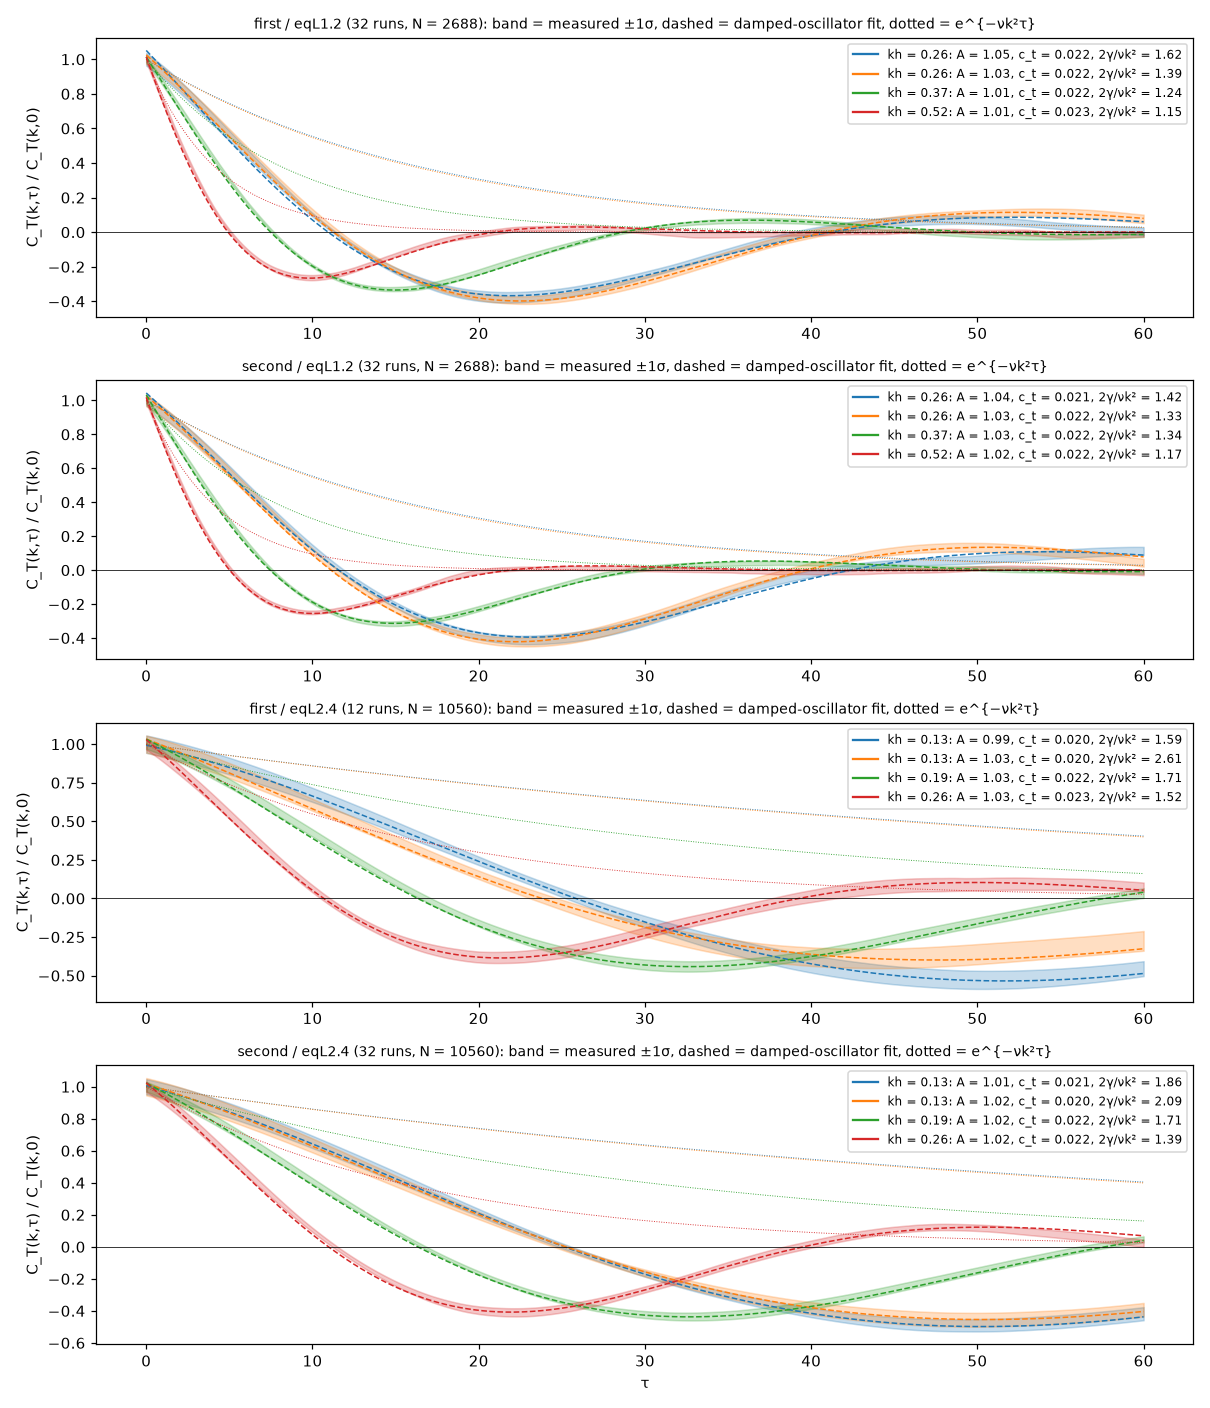
\includegraphics[width=\textwidth]{figs/transverse_fits.png}
\caption{$C_T(k,\tau)/C_T(k,0)$ to $\tau=60$ in the four smallest shells.  Band: measured
mean $\pm1\sigma$ over the realizations.  Dashed: fit of the damped oscillator,
\Eq{osc}.  Dotted: the hydrodynamic $e^{-\nu k^2\tau}$.  From top to bottom:
\texttt{first} and \texttt{second} at $L=1.2$ (32 runs each), \texttt{first} at $L=2.4$ (the 12
runs that finished) and \texttt{second} at $L=2.4$ (32 runs).  The legend gives the fitted
phase velocity $\omega/k$ and damping.}
\label{fig:tfits}
\end{figure}

\begin{figure}[t]
\centering
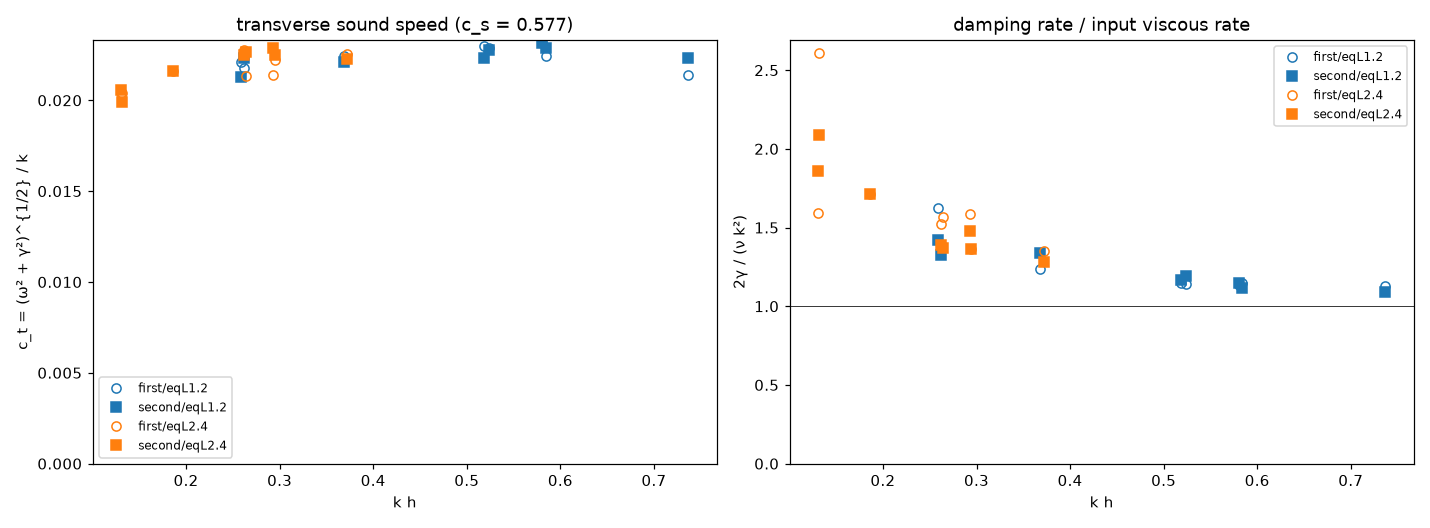
\includegraphics[width=\textwidth]{figs/transverse_dispersion.png}
\caption{The fits of \Fig{fig:tfits} in the eight smallest shells.  Left: the transverse
sound speed $c_t=(\omega^2+\gamma^2)^{1/2}/k$.  Right: the damping rate in units of the
viscous one, $2\gamma/\nu k^2$.  Blue: $L=1.2$; orange: $L=2.4$; open: \texttt{first},
filled: \texttt{second}.}
\label{fig:tdisp}
\end{figure}

\paragraph{\Fig{fig:tfits}: the transverse correlator is an oscillation.}  To long lags
$C_T$ crosses zero, reaches about $-0.4$, and comes back: it oscillates, at a frequency
proportional to $k$.  This is transverse sound, which a fluid does not have and an elastic
solid does.  The particles never melt at $\delta v=0.043$ (disorder $0.3a$), and the SPH
energy of a sheared lattice is not exactly that of the unsheared one, so the arrangement
responds as a weakly rigid solid.  The simplest model is a viscous fluid with a small shear
modulus $G$ (Kelvin--Voigt): the transverse displacement $u$ obeys
\st
\ddot u=-\nu k^2\dot u-c_t^2k^2u,\qquad c_t^2=\frac{G}{w},
\stp
and the momentum correlator is the velocity correlator of a damped oscillator,
\st
C_T(k,\tau)=A\,e^{-\gamma\tau}\Big[\cos\omega\tau-\frac{\gamma}{\omega}\sin\omega\tau\Big],
\qquad \gamma=\frac{\nu k^2}{2},\qquad \omega^2=c_t^2k^2-\gamma^2 .
\label{osc}
\stp
Its initial slope, $-2\gamma=-\nu k^2$, is the hydrodynamic one: at short lags the
oscillator and $e^{-\nu k^2\tau}$ agree, and they part once $c_tk\tau\sim1$.  We fit $A$,
$\gamma$ and $\omega$ in each shell.  The fits (dashed) lie on the data within the errors
over the whole range, with $A=1.0$--$1.07$.

\paragraph{\Fig{fig:tdisp}: what the fits give.}
\begin{itemize}
\item \emph{A constant transverse sound speed}, $c_t=0.022\pm0.001$ for $kh=0.13$--$0.74$,
  the same in both boxes and both campaigns: a linear dispersion, as for an elastic solid.
  Then
  \st
  \frac{G}{p}=\frac{w\,c_t^2}{p}=4c_t^2\approx2\times10^{-3}\qquad(w=4p),
  \stp
  a shear modulus three orders of magnitude below the pressure.  It is still large enough to
  dominate the shear mode at $kh\lesssim0.5$, where $c_tk>\nu k^2/2$, i.e.\ for
  \st
  k<\frac{2c_t}{\nu}\approx20,\qquad kh<1 .
  \stp
\item \emph{The damping is close to the viscous one at $kh\ge0.5$}: $2\gamma/\nu k^2=1.1$--$1.2$.
  At smaller $k$ it rises, to $1.3$--$1.5$ at $kh=0.26$ and $1.9$--$2.1$ at $kh=0.13$ (32 runs at
  $L=2.4$).  The fit recovers the damping of synthetic data to $\pm7\%$ with 8 runs
  (\Sect{sec:checks}), so this excess is real.  The extra rate,
  \st
  2\gamma-\nu k^2\approx0.015,\ 0.023,\ 0.036\qquad\text{at}\qquad kh=0.13,\ 0.26,\ 0.52,
  \stp
  grows roughly as $k^{2/3}$, not as $k^2$: it is not a viscosity.  Its origin is open
  (a slow relaxation of the arrangement, or the rise of $T$ over the run).
\item The two campaigns agree shell by shell: the oscillation is not an artifact of the
  start or of the code changes.
\end{itemize}
So the earlier statement that the effective shear viscosity is twice the input one at small
$k$ (\Fig{fig:corrL12}, right) is wrong: it was an exponential fitted to the onset of the
oscillation.  The viscosity is about right; what is wrong is the rigidity.

\subsection{The two campaigns side by side}
\label{sec:compare}

\paragraph{Purpose.}  \texttt{second} repeats the ensembles of \texttt{first} with the fast
code and the equilibrium start.  It checks the code changes on long runs and shows what the
start changes.

\begin{figure}[t]
\centering
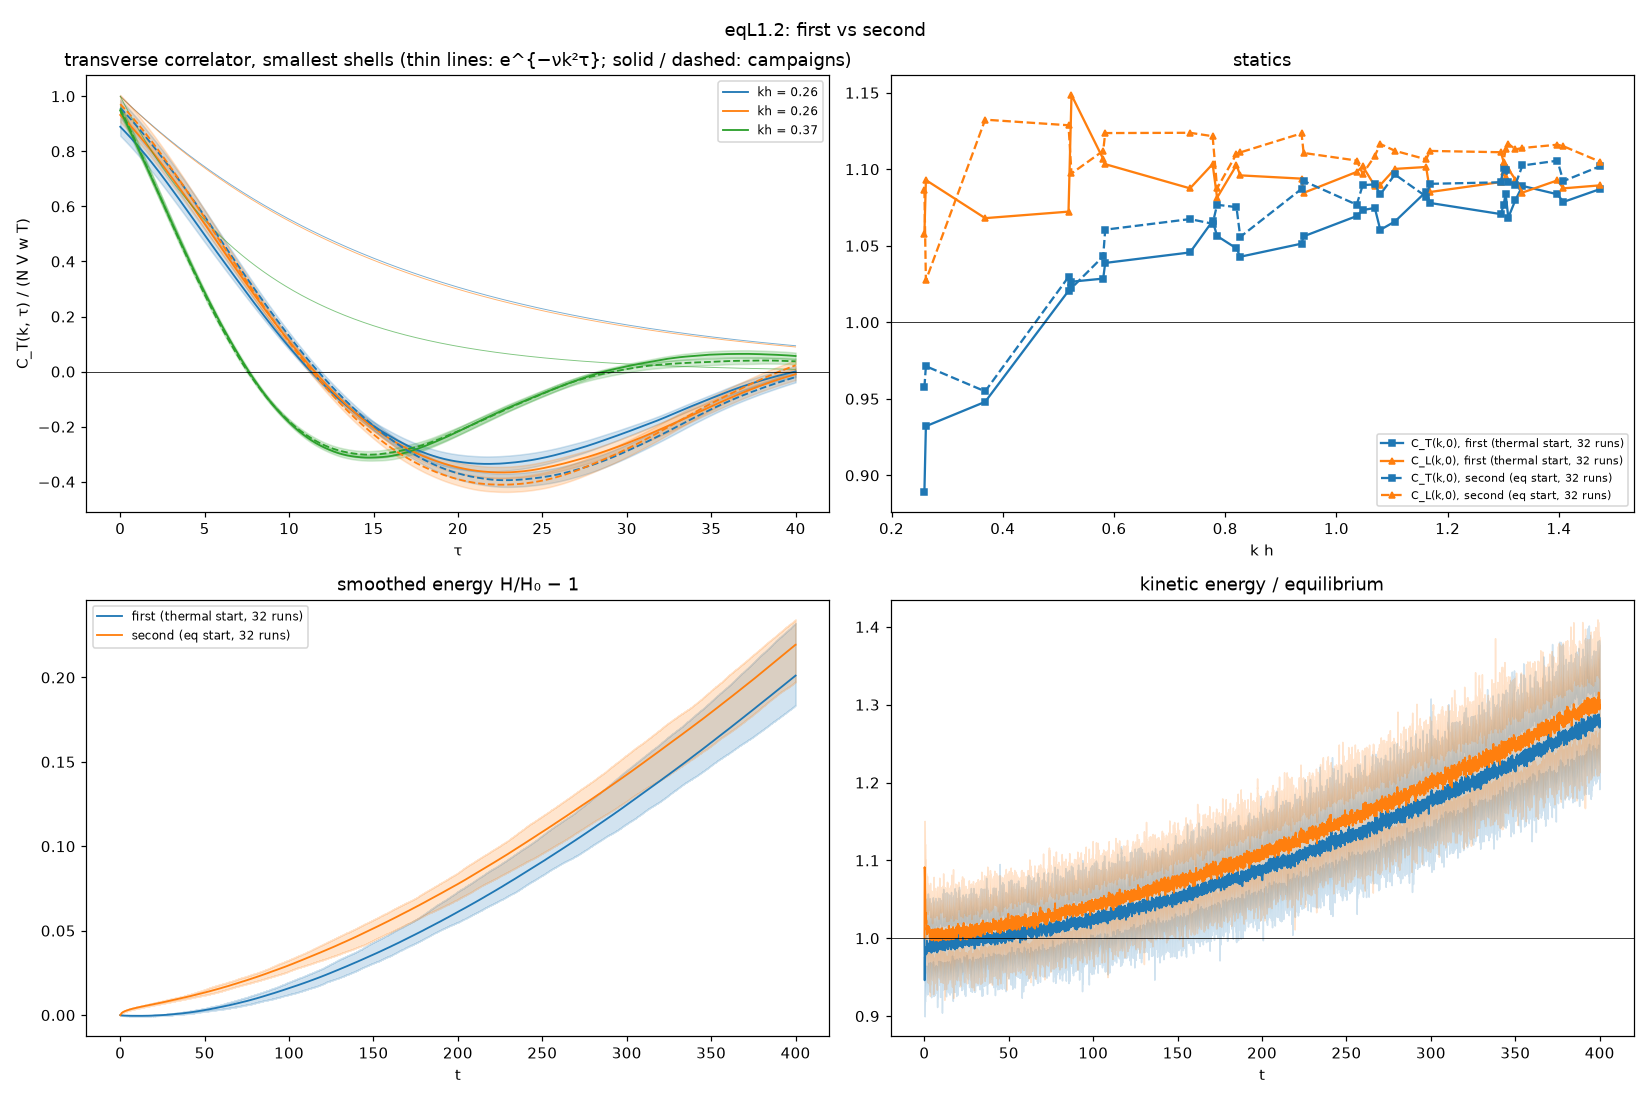
\includegraphics[width=\textwidth]{figs/compare_eqL1.2.png}
\caption{$L=1.2$, \texttt{first} (thermal start, old code, 32 runs) against \texttt{second}
(equilibrium start, fast code, 32 runs).  Top left: $C_T(k,\tau)$ in the three smallest
shells, solid \texttt{first}, dashed \texttt{second}, thin lines $e^{-\nu k^2\tau}$.  Top
right: the statics $C_T(k,0)$ (blue) and $C_L(k,0)$ (orange), normalized by the initial
$wT$.  Bottom: $H/H_0-1$ and the kinetic energy over its equilibrium value, mean over the
runs (line) and minimum to maximum (band).}
\label{fig:cmp12}
\end{figure}

\begin{figure}[t]
\centering
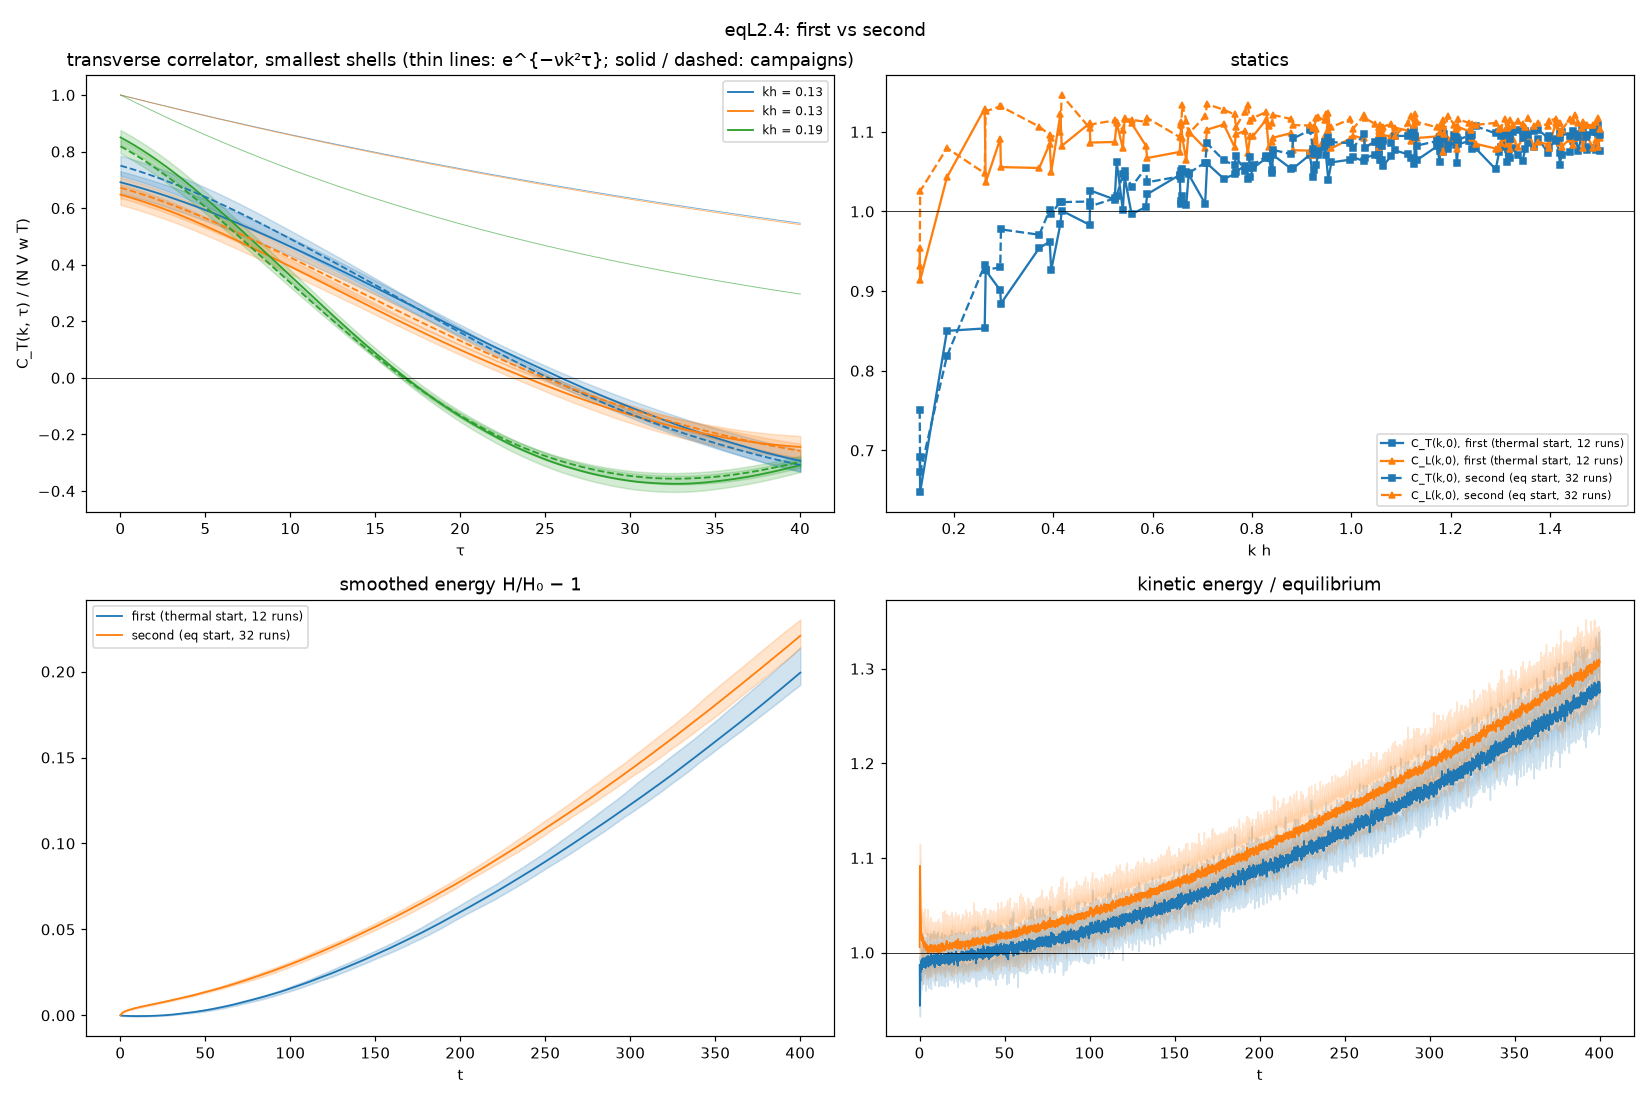
\includegraphics[width=\textwidth]{figs/compare_eqL2.4.png}
\caption{As \Fig{fig:cmp12} for $L=2.4$ ($N=10560$, smallest shell $kh=0.13$).
\texttt{first}: the 12 runs that finished; \texttt{second}: all 32.}
\label{fig:cmp24}
\end{figure}

\paragraph{What the figures show.}
\begin{center}
\begin{tabular}{lcccc}
\hline
 & runs & $H/H_0-1$ at $t=400$ & KE/eq at $t=400$ & $C_T(k,0)$, smallest shell \\ \hline
\texttt{first}, $L=1.2$ & 32 & $0.201\pm0.010$ & $1.28$ & $0.89$ \\
\texttt{second}, $L=1.2$ & 32 & $0.219\pm0.009$ & $1.31$ & $0.96$ \\
\texttt{first}, $L=2.4$ & 12 & $0.199\pm0.005$ & $1.28$ & $0.69$ ($kh=0.13$) \\
\texttt{second}, $L=2.4$ & 32 & $0.221\pm0.004$ & $1.31$ & $0.75$ ($kh=0.13$) \\
\hline
\end{tabular}
\end{center}
(the $\pm$ is the spread over the runs).
\begin{itemize}
\item \emph{The correlators agree.}  $C_T(k,\tau)$ is the same oscillation in both
  campaigns, and the statics agree within their scatter.  The fast code and the new start
  change nothing measurable in equilibrium.
\item \emph{The start.}  From the thermal start $H$ stays flat for $t\lesssim30$ and then heats
  (the particle energies start without fluctuations, \texttt{eqstart.tex}, which may be why); from the
  equilibrium start the heating begins at once.  By $t=400$ the two differ by $0.02$ in
  $H/H_0-1$, about two spreads.
\item \emph{The heating is the same in every box.}  $H/H_0-1\approx0.2$ and KE/eq $\approx1.3$
  at $t=400$, growing faster than linearly in time, as in the small box at the same $\delta
  v$ (\Sect{sec:stab}).  It is a property per particle, not of the box size.  Over the run
  $T$ rises by about $5\%$, which is why the statics at large $k$ sit at $1.05$--$1.10$.
\item \emph{The statics at small $k$} are low: $C_T(k,0)=0.89$--$0.96$ at $kh=0.26$ and
  $0.65$--$0.75$ at $kh=0.13$, and $C_L(k,0)\approx0.93$ at $kh=0.13$.  A possible cause is the
  rigidity: the runs start with the particles on the lattice, so the elastic energy of the
  long transverse modes starts at zero, and is filled only at the slow rate $\nu k^2$
  ($1/\nu k^2\approx70$ at $kh=0.13$), drawing on the kinetic energy.  The displacements are
  recorded in the runs now going, which will test this.
\end{itemize}

%=============================================================================
\section{Is the oscillation real?}
\label{sec:checks}

Three checks of the analysis (scripts on the branch \texttt{rigidity}).
\begin{enumerate}
\item \emph{An independent implementation.}  \texttt{examples/check\_correlators.py} reads the
  raw $M_T(\bm k,t)$ with h5py and computes $C_T$ by direct sums over $t$ (no FFT, no shared
  code).  For \texttt{second}, $L=1.2$, at $kh=0.26$ it gives $C_T=0.9575$, $0.5635$, $-0.3695$
  at $\tau=0$, $5$, $20$, the same to four digits as the Julia analysis.
\item \emph{Synthetic data.}  \texttt{test/testcorrelators.jl} generates transverse modes with
  a known shear modulus and viscosity,
  \st
  \dot u=v,\qquad dv=(-\nu k^2v-c_t^2k^2u)\,dt+\sqrt{2\nu k^2}\,dW,
  \stp
  sampled as in the runs (same $k$ shells, recording interval and length, 8 runs), and puts
  them through the same correlator and fit.
  \begin{center}
  \begin{tabular}{lccc}
  \hline
  input & $kh$ & $c_t$ fitted & $2\gamma/\nu k^2$ fitted \\ \hline
  $c_t=0.022$ & $0.26$, $0.37$, $0.52$ & $0.0220$, $0.0216$, $0.0219$ & $0.98$, $1.02$, $1.02$ \\
  $c_t=0$ (fluid) & $0.26$, $0.37$, $0.52$ & $0.000$, $0.000$, $0.003$ & $0.93$, $1.07$, $0.97$ \\
  \hline
  \end{tabular}
  \end{center}
  The analysis recovers both, and does not produce an oscillation from a fluid.
\item \emph{Physical controls}, running (\Sect{sec:next}): positions frozen (no Hamiltonian
  step), where $C_T$ must be $e^{-\nu k^2\tau}$; $\lambda=\infty$; and $c_t$ measured a second
  way, from the recorded displacements $u_T(\bm k,t)$, by
  \st
  c_t^2=\frac{\avg{|M_T|^2}}{(wV)^2k^2\avg{|u_T|^2}} .
  \stp
\end{enumerate}

%=============================================================================
\section{Random particle positions}
\label{sec:random}

If the rigidity comes from the hexagonal lattice, a random arrangement should not have it.
Short tests (box $0.6$, $t\le10$; positions uniform at random, the $s_a$ rescaled so that the
smoothed entropy is uniform, then the equilibrium start, which now handles unequal volumes):
\begin{center}
\begin{tabular}{lccc}
\hline
run & $t$ & KE/eq & $H/H_0-1$ \\ \hline
full scheme & $10$ & bursts to $150$ & $+0.64$, rising steadily \\
ideal SPH only & $5$ & $420$ & $10^{-4}$ (conserved) \\
stochastic step only, positions frozen & $5$ & $0.65$--$0.68$ & $10^{-4}$ \\
the same on the lattice & $5$ & $\approx1.0$ & $10^{-4}$ \\
\hline
\end{tabular}
\end{center}
At fixed particle entropies the SPH energy depends on the arrangement: the random one lies
about $400T$ per particle above the lattice, released as motion by the ideal step and turned
into heat by the viscous step.  So the equilibrium of the particle positions at temperature
$T$ is near a minimum of this energy, a solid, and a random arrangement is not an equilibrium
state at all.  In the continuum the energy of a perfect fluid is invariant under volume-preserving
relabelings of the fluid elements, which is why a fluid has no shear modulus; the SPH energy
breaks this symmetry at the scale $a$, by an amount set by the kernel's error on the lattice.
A fluid needs that breaking to be $\lesssim T$ per particle, or the particles to be relabeled
(moved relative to the fluid with the fields held fixed).

%=============================================================================
\section{Code changes between the campaigns}
\label{sec:code}

\paragraph{Speed.}  The serial parts (smoothing, velocities, Hamiltonian force,
thermodynamics, the bond weights) are threaded, the neighbour list is reused, and the
conformal equation of state is inverted in closed form.  Time per particle and step at
$L=2.4$:
\begin{center}
\begin{tabular}{lccc}
\hline
threads & 1 & 2 & 8 \\ \hline
before & $52\,\mu$s & $42\,\mu$s & $37\,\mu$s \\
after & $27\,\mu$s & $13\,\mu$s & $5.5\,\mu$s \\
\hline
\end{tabular}
\end{center}
Validation before \texttt{second}: 32 against 32 realizations ($L=0.6$, $t=50$), old against
new code; all 13 observables (KE/eq, $H/H_0-1$, the two acceptances, $C_{T,L}(k,0)$ and
$C_T(k,\tau=5)$ in three shells) agree within $1.3\sigma$.

\paragraph{Start.}  \texttt{second} starts from the equilibrium draw of
\texttt{eqstart.tex} (energies and momenta at one global $\beta^\mu$, totals shifted to the
target), so no thermalization is needed; \texttt{first} started from
\texttt{thermal\_init!} (momenta at fixed energies).

\paragraph{Checkpoints.}  Every 20 minutes the state goes to \texttt{<run>.chk} and the
record so far to the \texttt{.h5} (marked incomplete); resubmitting the task resumes it,
bit for bit.

%=============================================================================
\section{What we learned and open questions}
\label{sec:learned}

\begin{enumerate}
\item \emph{Stability.}  At $h/a=2$ the scheme with $\lambda=1$ is stable to $t=200$ for
  $\delta v\le0.078$ ($s_a\ge162$) and blows up at $\delta v=0.14$.  The blow-up needs the
  noise in the lattice modes: $\lambda=\infty$ never blows up.
\item \emph{Heating.}  All runs heat, at a rate $\propto\delta v^4$, $10$--$14$ times faster
  with $\lambda=1$ than with $\lambda=\infty$, and accelerating in time.  At $\delta v=0.043$
  it is $20\%$ in $H$ by $t=400$ in every box.  Its source is not identified.  A rate
  $\propto\delta v^4$ is second order in the fluctuations, as a time-step or
  representation error of the stochastic step would be.
\item \emph{Transverse sound.}  The particle arrangement has a shear modulus $G\approx2\times
  10^{-3}p$ ($c_t=0.022$).  It turns the shear mode into a damped oscillation for $kh\lesssim
  1$, which is the whole hydrodynamic range we can reach.  With it removed from the fit, the
  shear viscosity comes out $10$--$20\%$ above the input one at $kh\ge0.5$; at smaller $k$
  there is an extra damping that does not scale as $k^2$.
\item \emph{Code.}  The fast code and the equilibrium start reproduce the old ensembles.
\end{enumerate}

\paragraph{Next.}\label{sec:next}  Campaign \texttt{rigidity} (jobs 61045626, 61045885; $L=1.2$, $t=200$,
16 runs each, displacements recorded): $h/a=2$, $2.5$, $3$; the Wendland C4 kernel at $h/a=2$;
positions frozen; $\lambda=\infty$; and ideal SPH alone from the thermal start at each $h/a$.
How fast $c_t$ falls with $h/a$ and the kernel decides between a parameter choice and a change
of the scheme.

\paragraph{Open questions.}
\begin{enumerate}
\item Where does the rigidity come from, and how does it scale?  Candidates: the SPH
  energy of a sheared hexagonal lattice (a property of $H$ alone), or the stochastic step
  pinning the arrangement.  Tests: $c_t$ against $h/a$ and the kernel, in a run with the
  Hamiltonian step only (thermalized, no viscous step), and in a disordered (melted then
  cooled) arrangement.  If it comes from $H$, a larger $h/a$ should reduce it.
\item Where does the heating come from?  Tests: its dependence on $\Delta t$ (a step error
  falls as a power of $\Delta t$) and on $\eta/s$, with $\lambda=1$ and $\lambda=\infty$.
\item Why are $C_T(k,0)$, and less so $C_L(k,0)$, below one at the smallest $k$, and where does
  the extra damping $\propto k^{2/3}$ come from?
\item Which particle-energy variance is the equilibrium one in the particle representation,
  the drawn one or $9/16$ of it (\texttt{eqstart.tex})?
\end{enumerate}

\end{document}
